% Options for packages loaded elsewhere
\PassOptionsToPackage{unicode}{hyperref}
\PassOptionsToPackage{hyphens}{url}
\PassOptionsToPackage{dvipsnames,svgnames,x11names}{xcolor}
%
\documentclass[
  letterpaper,
  DIV=11,
  numbers=noendperiod]{scrartcl}

\usepackage{amsmath,amssymb}
\usepackage{lmodern}
\usepackage{setspace}
\usepackage{iftex}
\ifPDFTeX
  \usepackage[T1]{fontenc}
  \usepackage[utf8]{inputenc}
  \usepackage{textcomp} % provide euro and other symbols
\else % if luatex or xetex
  \usepackage{unicode-math}
  \defaultfontfeatures{Scale=MatchLowercase}
  \defaultfontfeatures[\rmfamily]{Ligatures=TeX,Scale=1}
  \setmainfont[]{Optima}
\fi
% Use upquote if available, for straight quotes in verbatim environments
\IfFileExists{upquote.sty}{\usepackage{upquote}}{}
\IfFileExists{microtype.sty}{% use microtype if available
  \usepackage[]{microtype}
  \UseMicrotypeSet[protrusion]{basicmath} % disable protrusion for tt fonts
}{}
\makeatletter
\@ifundefined{KOMAClassName}{% if non-KOMA class
  \IfFileExists{parskip.sty}{%
    \usepackage{parskip}
  }{% else
    \setlength{\parindent}{0pt}
    \setlength{\parskip}{6pt plus 2pt minus 1pt}}
}{% if KOMA class
  \KOMAoptions{parskip=half}}
\makeatother
\usepackage{xcolor}
\usepackage[top=30mm,left=30mm,heightrounded]{geometry}
\setlength{\emergencystretch}{3em} % prevent overfull lines
\setcounter{secnumdepth}{-\maxdimen} % remove section numbering
% Make \paragraph and \subparagraph free-standing
\ifx\paragraph\undefined\else
  \let\oldparagraph\paragraph
  \renewcommand{\paragraph}[1]{\oldparagraph{#1}\mbox{}}
\fi
\ifx\subparagraph\undefined\else
  \let\oldsubparagraph\subparagraph
  \renewcommand{\subparagraph}[1]{\oldsubparagraph{#1}\mbox{}}
\fi


\providecommand{\tightlist}{%
  \setlength{\itemsep}{0pt}\setlength{\parskip}{0pt}}\usepackage{longtable,booktabs,array}
\usepackage{calc} % for calculating minipage widths
% Correct order of tables after \paragraph or \subparagraph
\usepackage{etoolbox}
\makeatletter
\patchcmd\longtable{\par}{\if@noskipsec\mbox{}\fi\par}{}{}
\makeatother
% Allow footnotes in longtable head/foot
\IfFileExists{footnotehyper.sty}{\usepackage{footnotehyper}}{\usepackage{footnote}}
\makesavenoteenv{longtable}
\usepackage{graphicx}
\makeatletter
\def\maxwidth{\ifdim\Gin@nat@width>\linewidth\linewidth\else\Gin@nat@width\fi}
\def\maxheight{\ifdim\Gin@nat@height>\textheight\textheight\else\Gin@nat@height\fi}
\makeatother
% Scale images if necessary, so that they will not overflow the page
% margins by default, and it is still possible to overwrite the defaults
% using explicit options in \includegraphics[width, height, ...]{}
\setkeys{Gin}{width=\maxwidth,height=\maxheight,keepaspectratio}
% Set default figure placement to htbp
\makeatletter
\def\fps@figure{htbp}
\makeatother

\KOMAoption{captions}{tableheading}
\makeatletter
\makeatother
\makeatletter
\makeatother
\makeatletter
\@ifpackageloaded{caption}{}{\usepackage{caption}}
\AtBeginDocument{%
\ifdefined\contentsname
  \renewcommand*\contentsname{Table of contents}
\else
  \newcommand\contentsname{Table of contents}
\fi
\ifdefined\listfigurename
  \renewcommand*\listfigurename{List of Figures}
\else
  \newcommand\listfigurename{List of Figures}
\fi
\ifdefined\listtablename
  \renewcommand*\listtablename{List of Tables}
\else
  \newcommand\listtablename{List of Tables}
\fi
\ifdefined\figurename
  \renewcommand*\figurename{Figure}
\else
  \newcommand\figurename{Figure}
\fi
\ifdefined\tablename
  \renewcommand*\tablename{Table}
\else
  \newcommand\tablename{Table}
\fi
}
\@ifpackageloaded{float}{}{\usepackage{float}}
\floatstyle{ruled}
\@ifundefined{c@chapter}{\newfloat{codelisting}{h}{lop}}{\newfloat{codelisting}{h}{lop}[chapter]}
\floatname{codelisting}{Listing}
\newcommand*\listoflistings{\listof{codelisting}{List of Listings}}
\makeatother
\makeatletter
\@ifpackageloaded{caption}{}{\usepackage{caption}}
\@ifpackageloaded{subcaption}{}{\usepackage{subcaption}}
\makeatother
\makeatletter
\@ifpackageloaded{tcolorbox}{}{\usepackage[many]{tcolorbox}}
\makeatother
\makeatletter
\@ifundefined{shadecolor}{\definecolor{shadecolor}{rgb}{.97, .97, .97}}
\makeatother
\makeatletter
\makeatother
\ifLuaTeX
  \usepackage{selnolig}  % disable illegal ligatures
\fi
\IfFileExists{bookmark.sty}{\usepackage{bookmark}}{\usepackage{hyperref}}
\IfFileExists{xurl.sty}{\usepackage{xurl}}{} % add URL line breaks if available
\urlstyle{same} % disable monospaced font for URLs
\hypersetup{
  pdftitle={W4: Afrofuturism},
  colorlinks=true,
  linkcolor={blue},
  filecolor={Maroon},
  citecolor={Blue},
  urlcolor={Blue},
  pdfcreator={LaTeX via pandoc}}

\title{W4: Afrofuturism}
\author{}
\date{}

\begin{document}
\maketitle
\ifdefined\Shaded\renewenvironment{Shaded}{\begin{tcolorbox}[frame hidden, borderline west={3pt}{0pt}{shadecolor}, breakable, sharp corners, interior hidden, boxrule=0pt, enhanced]}{\end{tcolorbox}}\fi

\setstretch{1.2}
\begin{quote}
Unlike previous eras, today's artists can wield the power of digital
media, social platforms, digital video, graphic arts, gaming technology,
and more to tell their stories, share their stories, and connect with
audiences inexpensively---a gift from the sci-fi gods, so to speak, that
was unthinkable at the turn of the century. The storytelling gatekeepers
vanished with the high-speed modem, and for the first time in history,
people of color have a greater ability to project their own stories.
This tug-and-pull debate over black people controlling their image
shifts considerably when a fledgling filmmaker can shoot his sci-fi web
series on a \$500 DV cam, post it on YouTube, and promote it on
Instagram and Twitter.

---Ytasha L. Womack,
~\href{https://ebookcentral.proquest.com/lib/emerson/reader.action?docID=1381831\&ppg=1}{\emph{Afrofuturism:
The World of Black Sci-Fi and Fantasy Culture}}: 10.

What I like about Afrofuturism is it helps create our own space in the
future; it allows us to control our imagination . . . An Afrofuturist is
not ignorant of history, but they don't let history restrain their
creative impulses either.

---Raynaldo Anderson, cited in Ytasha Womack, \emph{Afrofuturism}
\end{quote}

\begin{center}\rule{0.5\linewidth}{0.5pt}\end{center}

\hypertarget{i.-angels-of-history}{%
\subsubsection{I. Angels of History}\label{i.-angels-of-history}}

\begin{figure}

\begin{minipage}[t]{0.49\linewidth}

{\centering 

\raisebox{-\height}{

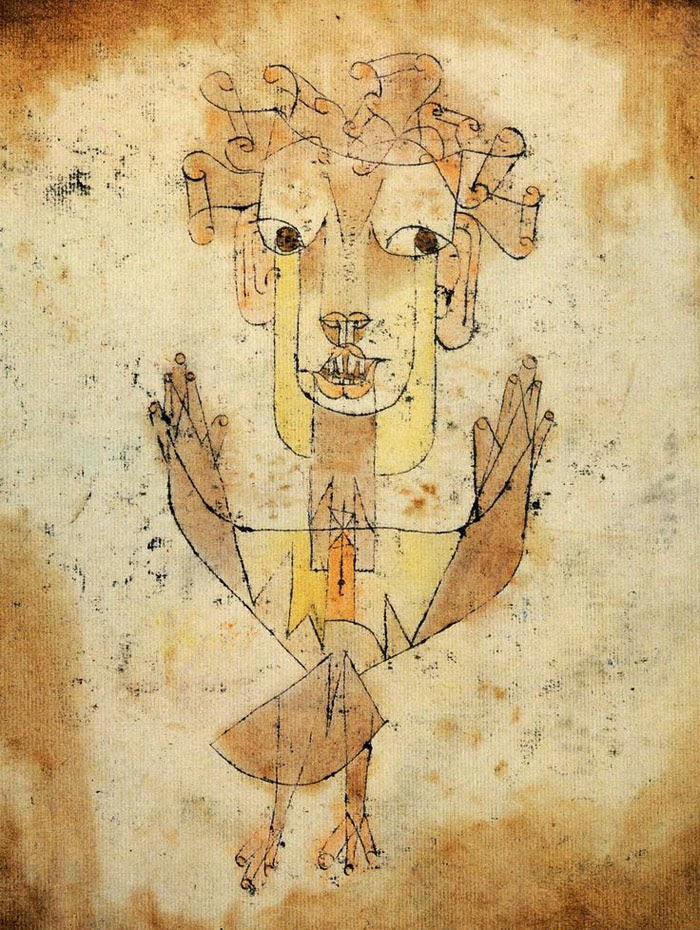
\includegraphics{../img/angelus-novus.jpg}

}

\caption{Paul Klee, ``Angelus Novus,'' 1920}

}

\end{minipage}%
%
\begin{minipage}[t]{0.02\linewidth}

{\centering 

~

}

\end{minipage}%
%
\begin{minipage}[t]{0.49\linewidth}

{\centering 

A Klee drawing named ``Angelus Novus'' shows an angel looking as though
he is about to move away from something he is fixedly contemplating. His
eyes are staring, his mouth is open, his wings are spread. This is how
one pictures the angel of history. His face is turned toward the past.
Where we perceive a chain of events, he sees one single catastrophe that
keeps piling ruin upon ruin and hurls it in front of his feet. The angel
would like to stay, awaken the dead, and make whole what has been
smashed. But a storm is blowing from Paradise; it has got caught in his
wings with such violence that the angel can no longer close them. The
storm irresistibly propels him into the future to which his back is
turned, while the pile of debris before him grows skyward. This storm is
what we call progress.---Walter Benjamin, ``Theses on the Philosophy of
History'' (1939), in \emph{Illuminations: Essays and Reflections}.
Edited and with an introduction by Hannah Arendt (New York: Schocken
Books, 1969).

}

\end{minipage}%

\end{figure}

\begin{center}\rule{0.5\linewidth}{0.5pt}\end{center}

Jason Farago,
``\href{https://www.bbc.com/culture/article/20160401-how-klees-angel-of-history-took-flight}{How
Klee's `Angel of History' Took Flight}'' (BBC Culture, 6 April 2016)

\begin{center}\rule{0.5\linewidth}{0.5pt}\end{center}

\emph{The Last Angel of History} (John Akomfrah/Black Audio Film
Collective, 1995)

Mark Dery,
``\href{https://canvas.emerson.edu/courses/1932613/files/145602338?wrap=1}{Black
to the Future: Interviews with Samuel R. Delaney, Greg Tate, and Tricia
Rose},'' in \emph{Flame Wars: The Discourse of Cyberculture} (Durham:
Duke University Press, 1994.

Kodwo Eshun,
``\href{https://canvas.emerson.edu/courses/1932613/files/145602336?wrap=1}{Further
Considerations on Afrofuturism}'' \emph{The New Centennial Review},
vol.~3, no. 2, Summer2003, pp.~287-302.

\textbf{Films}

\emph{Space Is The Place} (Sun Ra, 1974)

\emph{The Last Angel of History} (John Akomfrah, 1996)

\href{https://www.justwatch.com/us/movie/hidden-figures}{\emph{Hidden
Figures}} (Theodore Melfi, 2016)

\href{https://www.smithsonianchannel.com/special/afrofuturism-the-origin-story}{\emph{Afrofuturism:
The Origin Story}} (Smithsonian Channel, 2022)

\emph{Black Panther} (Ryan Coogler, 2018); \emph{Black Panther: Wakanda
Forever} (Ryan Coogler, 2022)

\textbf{References}

Paul Gilroy, \emph{The Black Atlantic: Modernity and Double
Consciousness} (Cambridge: Harvard University Press, 1993).

Kodwo Eshun, \emph{More Brilliant Than The Sun: Adventures in Sonic
Fiction} (London: Quartet Books, 1998).

Ytasha L. Womack,
\href{https://ebookcentral.proquest.com/lib/emerson/reader.action?docID=1381831\&ppg=1}{\emph{Afrofuturism:
The World of Black Sci-Fi and Fantasy Culture}} (Chicago: Lawrence Hill
Books, 2013).

\begin{center}\rule{0.5\linewidth}{0.5pt}\end{center}

\hypertarget{ii.-digital-afrofuturism}{%
\subsubsection{II. Digital
Afrofuturism}\label{ii.-digital-afrofuturism}}

\href{https://www.manzel.biz/gallery}{\includegraphics{w4-afrofuturism_files/mediabag/preview.pdf}}~~

``\href{https://www.africandigitalart.com/the-futurist-digital-collages-by-manzel-bowman/}{The
Futurist Digital Collages by Manzel Bowman}''
(\href{http://africandigitalart.com}{African Digital Art})

\begin{figure}

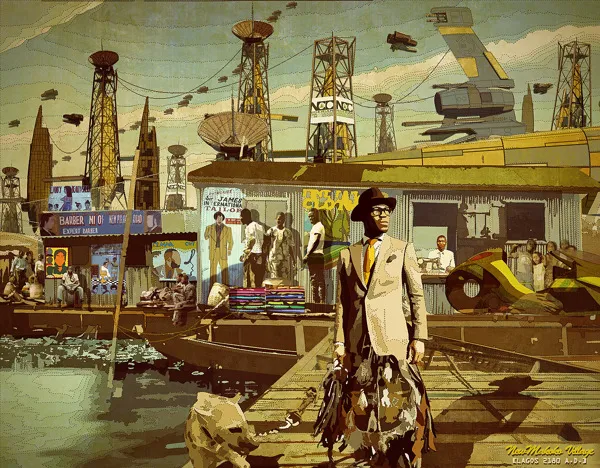
\includegraphics{../img/lagos-2180.jpg} \hfill{}

\caption{Olalekan Jeyifous, ``Lagos 2180 AD'' (2013)}

\end{figure}

\href{https://jeyifo.us/SMS}{Olalekan Jeyifous, Shanty Mega-Structures}

\begin{center}\rule{0.5\linewidth}{0.5pt}\end{center}

\hypertarget{iii.-feminist-afrofutures}{%
\subsubsection{III. Feminist
Afrofutures}\label{iii.-feminist-afrofutures}}

\begin{figure}

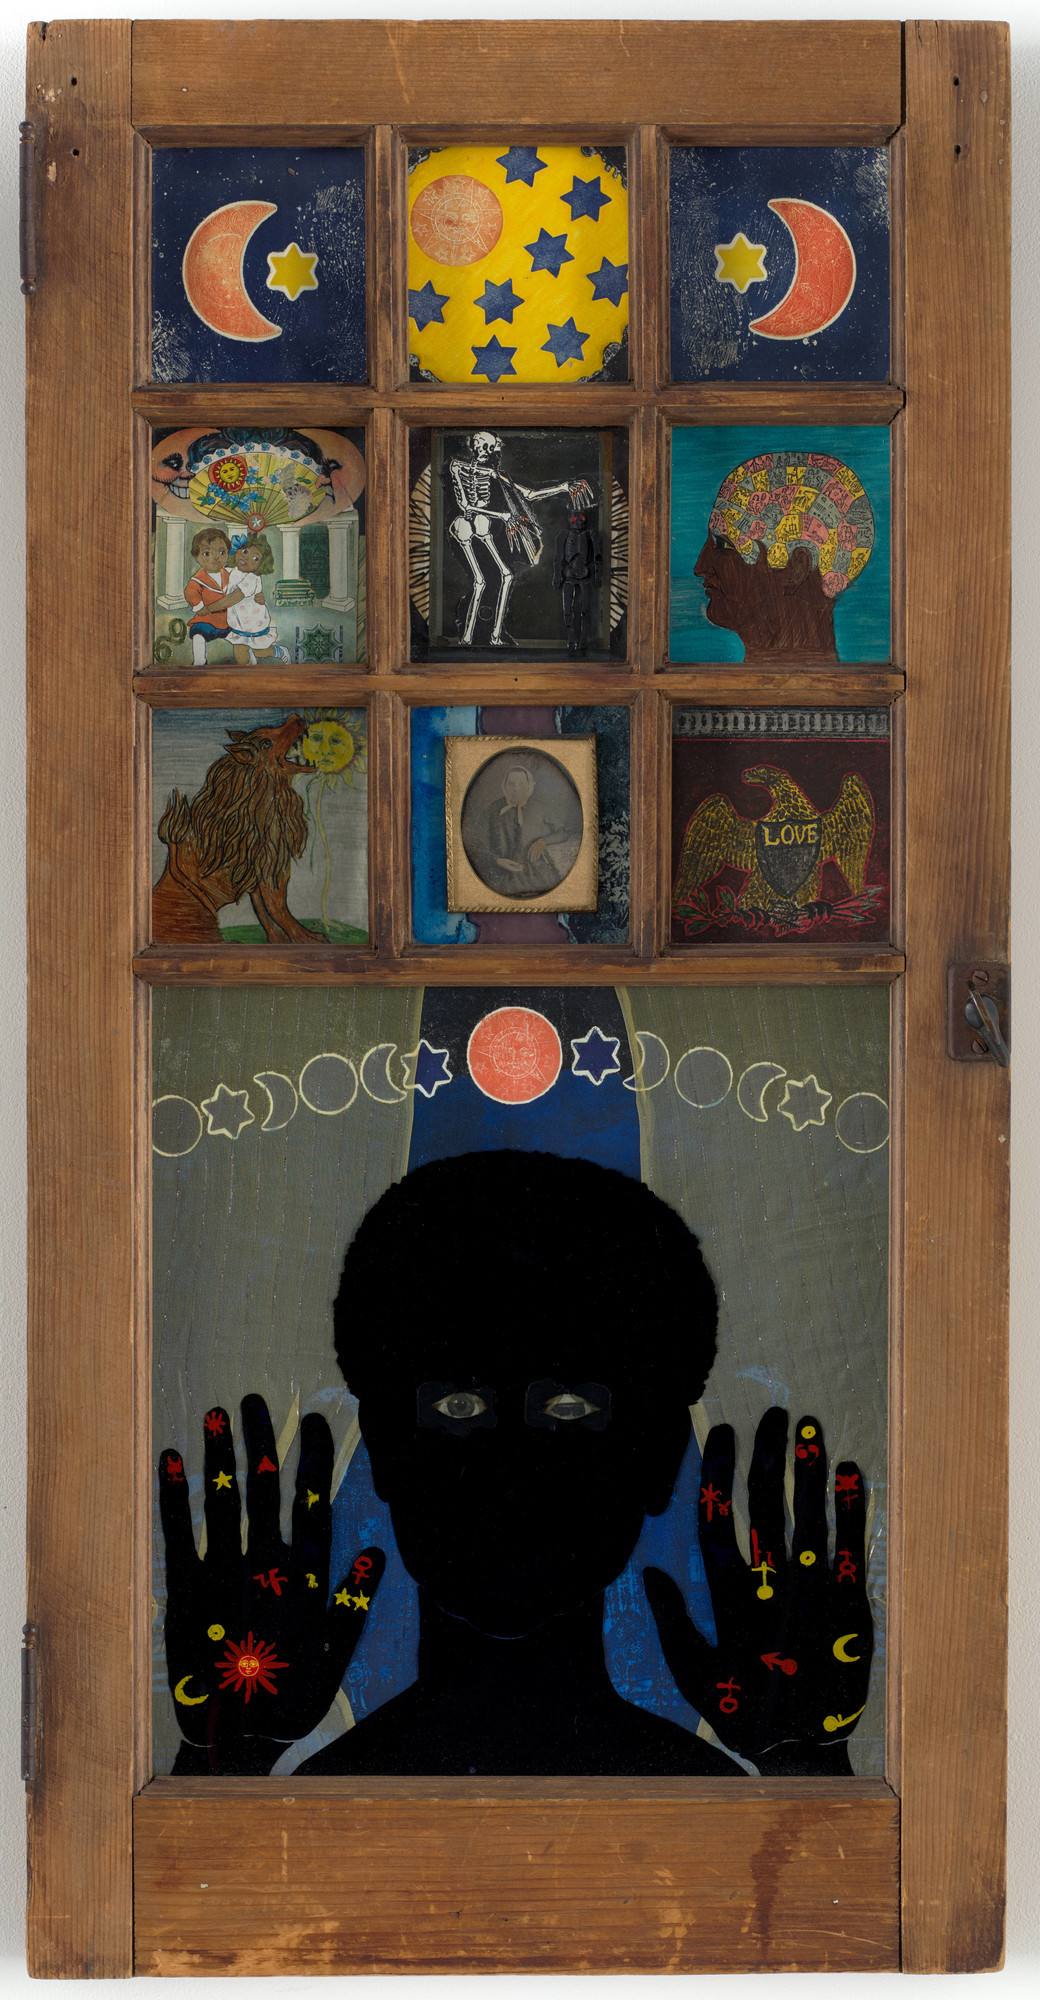
\includegraphics[width=4.16667in,height=\textheight]{../img/betye-saar.jpg} \hfill{}

\caption{Betye Saar, ``Black Girl's Window'' (1969)}

\end{figure}

Nicole D. Sconiers,
``\href{http://nicolesconiers.com/blog/2012/02/20/the-state-of-black-sci-fi-2012-my-tribute-to-afrofuturist-betye-saar/}{The
State of Black Sci-Fi 2012: My Tribute to Afrofuturist Betye Saar}''

Martine Syms,
``\href{http://thirdrailquarterly.org/martine-syms-the-mundane-afrofuturist-manifesto/}{The
Mundane Afrofuturist Manifesto}'' (2013)

\url{https://youtu.be/otUJvQhCjJ0}

\url{https://youtu.be/mXR4IaUmpZk}

\href{https://mubi.com/films/the-african-desperate}{\emph{The African
Desperate}}~(Martine Syms, 2022). Currently streaming on MUBI and Apple
TV



\end{document}
